\documentclass{article}


\usepackage{fancyhdr}
\usepackage{extramarks}
\usepackage{amsmath}
\usepackage{amsthm}
\usepackage{amsfonts}
\usepackage{tikz}
\usepackage[plain]{algorithm}
\usepackage{algpseudocode}
\usepackage{enumerate}
\usepackage{tikz}
\usepackage{listings}
\usepackage{hyperref}
\usepackage{subfigure}
\usepackage[graphicx]{realboxes}
\usepackage{xcolor}
\usepackage{color}



% 代码块高级设置
\lstset{
basicstyle=\footnotesize,                 % 设置整体的字体大小
showstringspaces=false,                     % 不显示字符串中的空格
frame=single,                               % 设置代码块边框
numbers=left,                               % 在左侧显示行号
% numberstyle=\footnotesize\color{gray},    % 设置行号格式
numberstyle=\color{darkgray},               % 设置行号格式
backgroundcolor=\color{white},              % 设置背景颜色
keywordstyle=\color{blue},                  % 设置关键字颜色
commentstyle=\it\color[RGB]{0,100,0},       % 设置代码注释的格式
stringstyle=\sl\color{red},                 % 设置字符串格式
}

\hypersetup{hidelinks,
	colorlinks=true,
	allcolors=black,
	pdfstartview=Fit,
	breaklinks=true}

%
% Basic Document Settings
%  

\topmargin=-0.45in
\evensidemargin=0in
\oddsidemargin=0in
\textwidth=6.5in
\textheight=9.0in
\headsep=0.25in

\linespread{1.1}

\pagestyle{fancy}
\lhead{}
\chead{\hmwkClass : \hmwkTitle}
\rhead{\firstxmark}
\lfoot{\lastxmark}
\cfoot{\thepage}

\renewcommand\headrulewidth{0.4pt}
\renewcommand\footrulewidth{0.4pt}

\setlength\parindent{0pt}



%
% Homework Details
%   - Title
%   - Due date
%   - Class
%   - Instructor
%   - Class number
%   - Name
%   - Student ID

\newcommand{\hmwkTitle}{Problem Set 3 Document}
\newcommand{\hmwkDueDate}{Dec 5th}
\newcommand{\hmwkClass}{Parallel Computing}
\newcommand{\hmwkClassInstructor}{Professor Rui Fan}

% 正式选课名单确定之后,根据通知填写所在班级编号

\newcommand{\hmwkAuthorName}{Zhenghong Yu}
\newcommand{\hmwkAuthorMail}{yuzhh1@shanghaitech.edu.cn}
\newcommand{\hmwkAuthorID}{2020533156}


%
% Title Page
%

\title{
    \vspace{2in}
    \textmd{\textbf{\hmwkClass:\\  \hmwkTitle}}\\
    \normalsize\vspace{0.1in}\small{Due\ on\ \hmwkDueDate\ at 23:59 }\\
   \vspace{2in}
}

\author{
    Mailbox: \hmwkAuthorMail\\
	Student ID: \hmwkAuthorID\\
    Student Name: \hmwkAuthorName}
\date{}




\begin{document}

\maketitle
\pagebreak
\tableofcontents

\pagebreak





\section{Problem 1}
Consider the same situation as in problem 1 of problem set 2. Give another 
algorithm for all-to-all broadcast which takes time $(t_{s} + t_{w}m) (p-1)$.\\
Hint: Try to embed a $p$ process ring in the tree.\\
\textbf{Solution: }\\
I use Euler-tour representation to traverse the tree to be a ring. Here is a sample on a tree
\begin{center}
    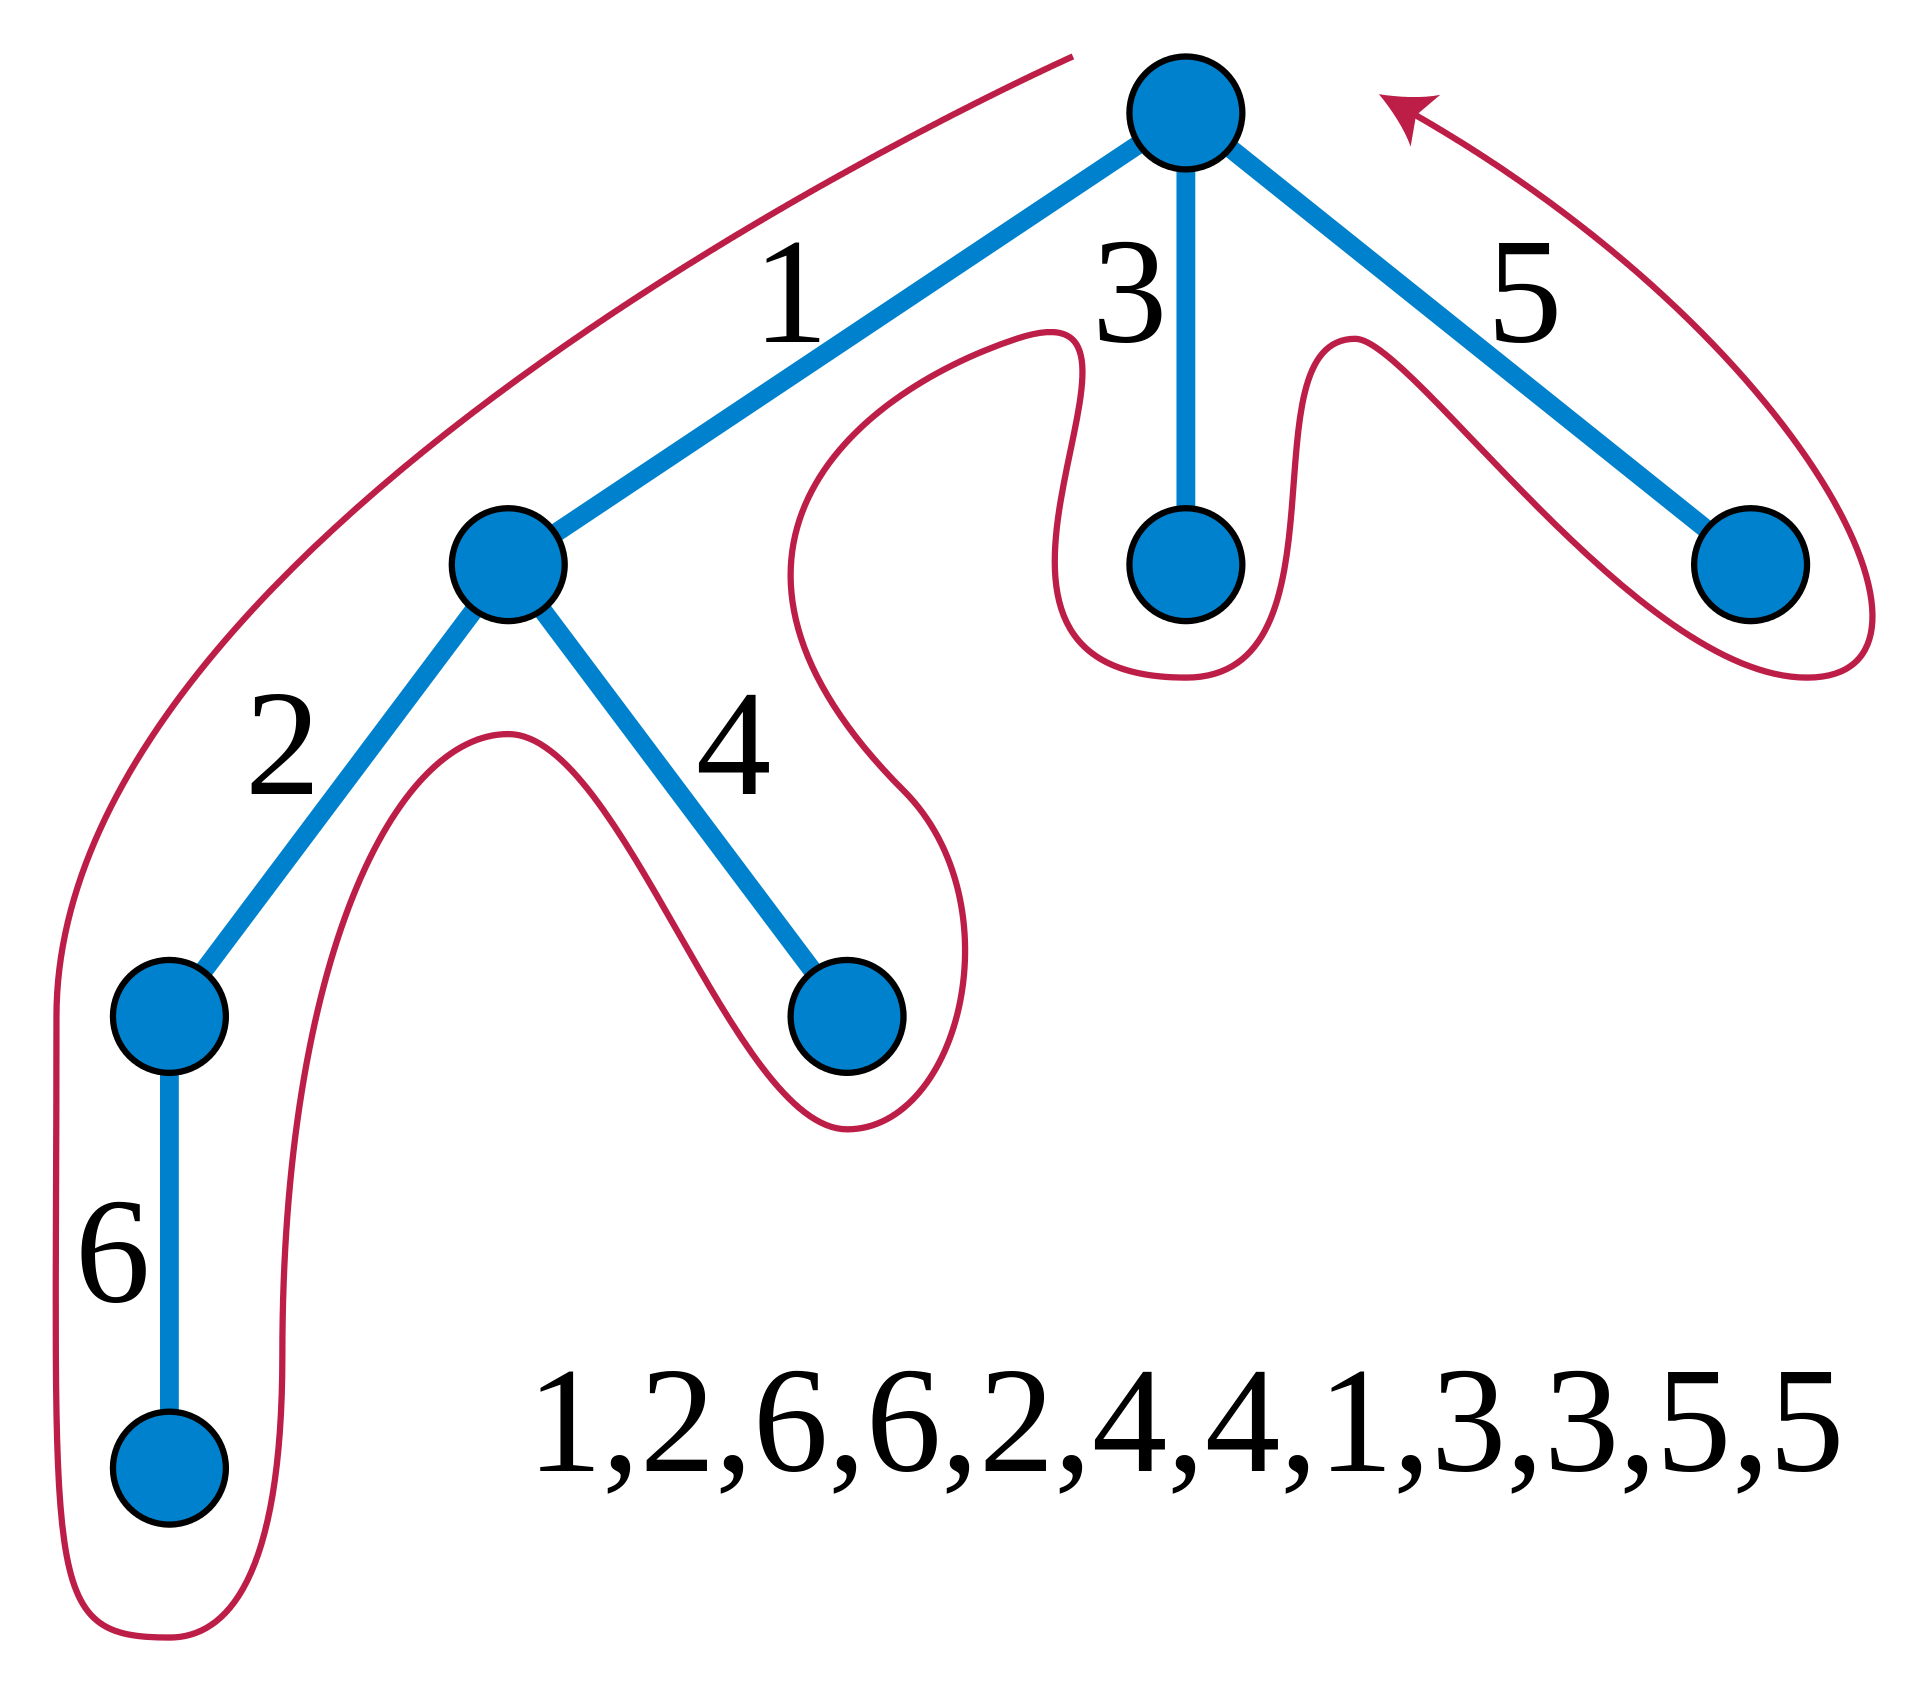
\includegraphics[scale = 0.09]{6.png}\\
\end{center}
With applying the ring-broadcast method, it will make the workload of every single directional channel to be $m$. Therefore, the time cost should be $(t_{s}+t_{w}m)(p-1)$.
\section{Problem 2}
We discussed barrier synchronization as a way to ensure all threads reach a point 
in the code before any of them progress beyond the point. The figure below 
shows a barrier for N threads implemented using locks. Explain clearly how 
this code works. What should the initial values of count and the arrival and 
deparoure locks be? Why is it necessary to use two lock variables? 
\begin{center}
    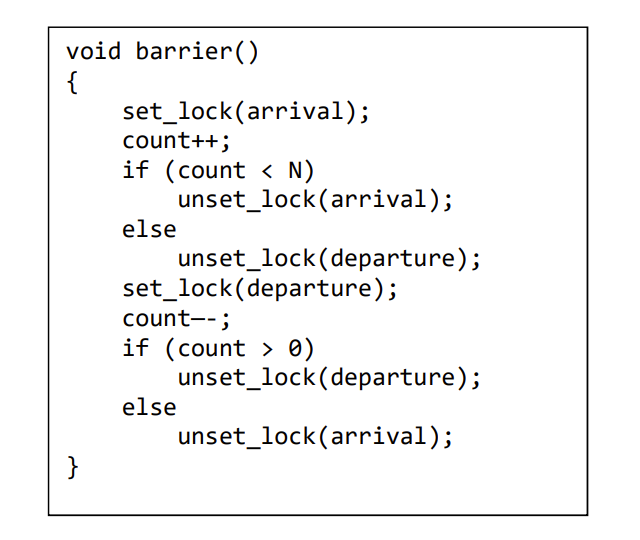
\includegraphics[scale = 0.4]{1.png}\\
\end{center}
\textbf{Solution:}\\
The initial value of \textbf{count} should be 0, \textbf{arrival} should be unset, \textbf{departure} should be set.\\
The \textbf{arrival} lock make sure that the variable \textbf{count} to be increased by only one thread at the same time. Once a thread get \textbf{arrival} lock, increase count, if not all threads are arrival, the \textbf{arrival} lock will be released, and then thread will try to access \textbf{departure} lock. If the thread is the last one to arrival, the \textbf{departure} lock will be released. Thus, all not last thread will wait at setting \textbf{departure} lock until the last thread release it. All thread synchronization.\\
The \textbf{departure} lock protect variable \textbf{count} to be decreased by only one thread at the same time. Similarly, after all thread leave, the \textbf{arrival} lock will be released and the barrier will be back to the previous state.\\
The two lock is used to protect increment and decreasement atomatically to prevent more than one thread do the things which should only done by the last thread.

\section{Problem 3}
\subsection{Question 1}
Consider the sequential code shown in the figure below. List all the dependence 
relationships in the code, indicating the type of dependence in each case. Draw 
the loop-carried dependence graph (LDG).
\begin{center}
    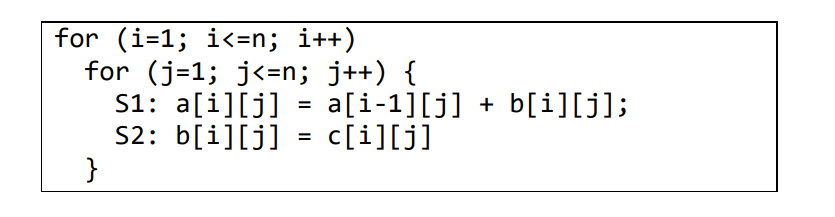
\includegraphics[scale = 0.4]{2.png}\\
\end{center}
\textbf{Solution:}\\
Dependences:
\begin{itemize}
    \item $S_{1}[i,j]\rightarrow TS_{1}[i+1,j]$
    \item $S_{1}[i,j]\rightarrow AS_{2}[i,j]$
\end{itemize} 
\begin{center}
    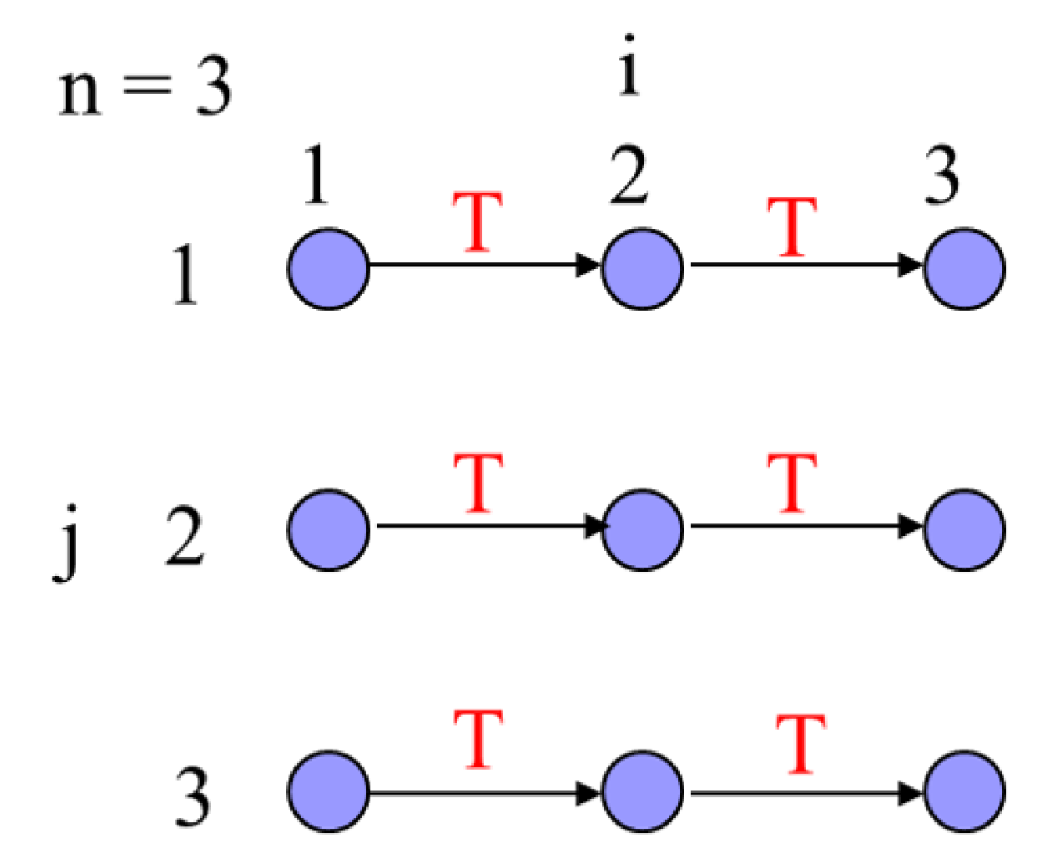
\includegraphics[scale = 0.25]{3.png}\\
\end{center}
\subsection{Question 2}
Using the LDG derived in Q1a, describe how to obtain a parallel algorithm, 
explaining any modifications required to improve the efficiency. Express your 
parallel algorithm using OpenMP. 
\\\textbf{Solution:}\\
Since we can see that there is no dependences between $j$, I choose to put $j$ to outer iteration.
\begin{lstlisting}[language=c++]
#pragma omp parrallel for private(i) schedule(dynamic)
for (j=1; j<=n; j++) {
    for (i=1; i<=n; i++) {
        S1: a[i][j] = a[i-1][j] + b[i][j];
        S2: b[i][j] = c[i][j];
    }
}
\end{lstlisting}


\section{Problem 4}
Consider the loop shown in the figure below. Indicate the loop-carried 
dependence relationships. By restructuring the code, is it possible to eliminate 
this dependence and parallelize the loop? Express your answer using OpenMP.
\begin{center}
    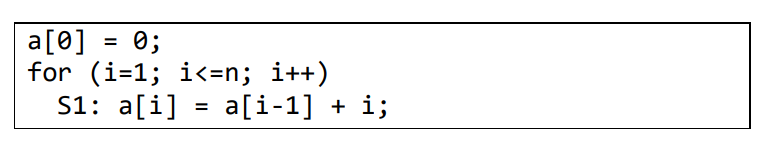
\includegraphics[scale = 0.4]{4.png}\\
\end{center}
\textbf{Solution:}\\
Dependences:
\begin{itemize}
    \item $S_{1}[i]\rightarrow TS_{1}[i+1]$
\end{itemize}
But when we observe it, we can conclude that each $a[i]=0+1+2+3+\cdots+i=\frac{(1+i)i}{2}$,so
\begin{lstlisting}[language=c++]
a[0] = 0;
#pragma omp parrallel for schedule(dynamic)
for (i=1; i<=n; i++) {
    a[i] = i * (i+1) / 2;
}
\end{lstlisting}

\section{Problem 5}
One way to get a numerical approximation to $\pi$ is to sum the following 
sequence: 
$$\pi=4(1-\frac{1}{3}+\frac{1}{5}-\frac{1}{7}+\cdots)$$
A sequential algorithm to calculate $\pi$ using this formula is given in the figure 
below. By analyzing the loop-carried dependences in this code, show how the 
algorithm may be parallelized, expressing your answer using OpenMP. Indicate 
clearly any modifications required to the code in order to allow parallelization 
and improve the efficiency. 
\begin{center}
    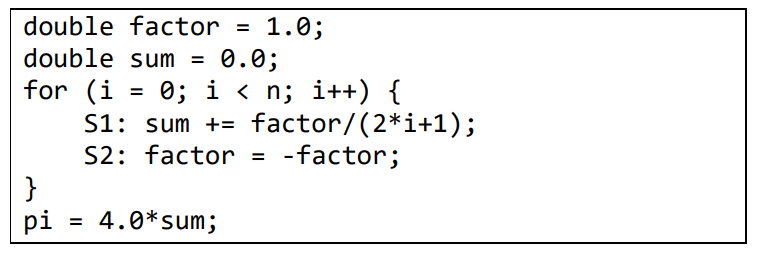
\includegraphics[scale = 0.4]{5.png}\\
\end{center}
\textbf{Soltion:}\\
Dependences:
\begin{itemize}
    \item $S_{1}[i]\rightarrow TS_{1}[i+1]$
    \item $s_{2}[i]\rightarrow TS_{2}[i+1]$
    \item $S_{2}[i]\rightarrow TS_{1}[i+1]$
\end{itemize}
\begin{lstlisting}[language=c++]
double factor = 0.0;
double sum = 0.0;
#pragma omp parrallel for private(factor) reduction(+:sum) schedule(dynamic)
for (i=0; i<n; i++) {
    if(i%2)
    {
        factor = 1;
    }
    else
    {
        factor = -1;
    }
    sum += factor / (2 * i + 1);
}
pi = 4.0 * sum;
\end{lstlisting}
\end{document}
